\documentclass{article}

\usepackage{graphicx}
\usepackage{tikz}
\usepackage{tikzsymbols}
\usetikzlibrary{calc,patterns,shapes.geometric}
\pagestyle{empty}
\usepackage[margin=0pt]{geometry}
\geometry{papersize={14in,12in}}

\def\centerarc[#1](#2)(#3:#4:#5){\draw[#1] ($(#2)+({#5*cos(#3)},{#5*sin(#3)})$) arc (#3:#4:#5);}

\begin{document}
	\begin{figure}
		\centering
		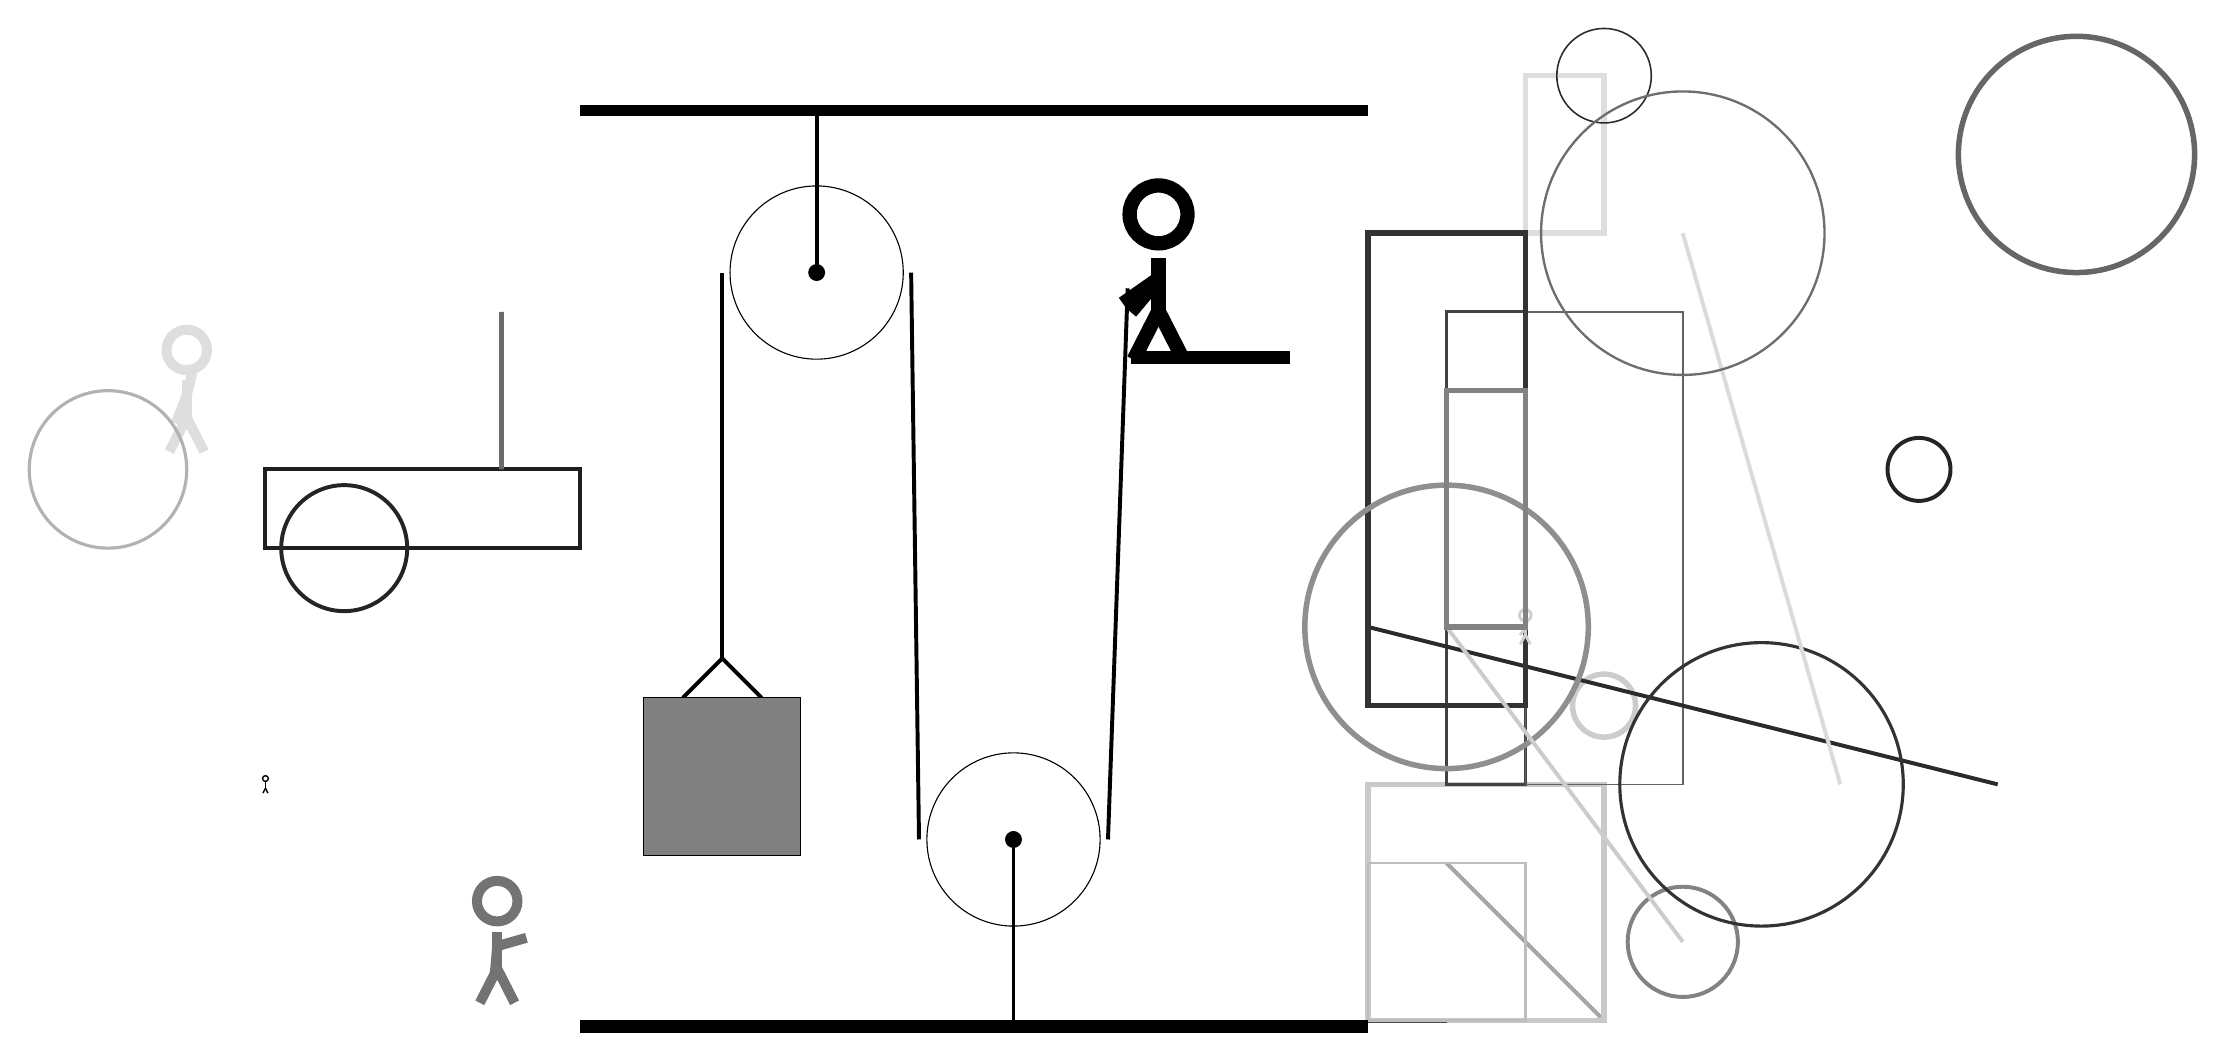
\begin{tikzpicture}
			%%%%% START %%%%%
			
			\draw[fill=black] (-2, 11.5) rectangle (8, 11.625);
			
			\draw (3.5, 2.3) circle (1.1);
			\draw[fill=black] (3.5, 2.3) circle (0.1);
			\draw[line width=0.5mm] (3.5, 2.3) -- (3.5, 0);
			
			\draw (1, 9.5) circle (1.1);
			\draw[fill=black] (1, 9.5) circle (0.1);
			\draw[line width=0.5mm] (1, 11.5) -- (1, 9.5);
			
			\draw[line width=0.5mm, color=black!35](11, 0) -- (9, 2);
			
			\draw[line width=0.7mm, color=black!13] (10, 10) rectangle (11, 12);
			\draw[line width=0.7mm, color=black!21] (8, 3) rectangle (11, 0);
			\draw[line width=0.4mm, color=black!74] (10, 3) rectangle (9, 9);
			\draw[line width=0.2mm, color=black!61] (10, 9) rectangle (12, 3);
			\draw [line width=0.5mm, color=black!49](12, 1) circle (0.7);
			
			\node[line width=0.3mm, color=black!98] at (-6, 3) {\Strichmaxerl[1][90][90]};
			\draw[line width=0.5mm, color=black!71](9, 0) -- (8, 0);
			\draw[line width=0.5mm, color=black!88] (-2, 7) rectangle (-6, 6);
			\draw[line width=0.3mm, color=black!26] (10, 0) rectangle (8, 2);
			
			\draw [line width=0.7mm, color=black!20](11, 4) circle (0.4);
			
			\draw[line width=0.5mm, color=black!83](8, 5) -- (16, 3);
			\draw [line width=0.5mm, color=black!86](-5, 6) circle (0.8);
			\node[line width=0.6mm, color=black!55] at (-3, 1) {\Strichmaxerl[7][85][16]};
			\draw [line width=0.5mm, color=black!86](15, 7) circle (0.4);
			\draw [line width=0.4mm, color=black!80](13, 3) circle (1.8);
			
			\draw[line width=0.5mm, color=black!14](12, 10) -- (14, 3);
			\node[line width=0.3mm, color=black!13] at (-7, 8) {\Strichmaxerl[7][69][76]};
			\draw [line width=0.2mm, color=black!83](11, 12) circle (0.6);
			\draw[line width=0.7mm, color=black!80] (8, 10) rectangle (10, 4);
			\draw [line width=0.7mm, color=black!44](9, 5) circle (1.8);
			
			\draw [line width=0.7mm, color=black!60](17, 11) circle (1.5);
			\draw [line width=0.4mm, color=black!30](-8, 7) circle (1.0);
			\draw[line width=0.5mm, color=black!20](9, 5) -- (12, 1);
			\node[line width=0.2mm, color=black!19] at (10, 5) {\Strichmaxerl[2][53][74]};
			
			\draw[line width=0.6mm, color=black!58] (-3, 7) rectangle (-3, 9);
			\draw[line width=0.7mm, color=black!49] (9, 5) rectangle (10, 8);
			\draw [line width=0.3mm, color=black!57](12, 10) circle (1.8);
			
			\draw[line width=0.5mm](-0.7, 4.1) --  (-0.2, 4.6) -- (0.3, 4.1);
			\draw[fill=black!50] (-1.2, 4.1) rectangle (0.8, 2.1);
			
			\draw[line width=0.5mm](-0.2, 9.5) -- (-0.2, 4.6);
			\centerarc[line width=0.5mm](1, 9.5)(180:0:1.2000000000000002)
			\draw[line width=0.5mm](2.2, 9.5) -- (2.3, 2.3);
			\centerarc[line width=0.5mm](3.5, 2.3)(180:360:1.2000000000000002)
			\draw[line width=0.5mm](4.7, 2.3) -- (4.95, 9.3);
			
			\node at (5.3, 9.5) {\Strichmaxerl[10][35][-130]};
			\draw[fill=black] (5, 8.5) rectangle (7, 8.35);
			
			\draw[fill=black] (-2, 0) rectangle (8, -0.15);
			
			%%%%% END %%%%%
		\end{tikzpicture}
	\end{figure}	
\end{document}